\documentclass[a4paper, 11pt, oneside, polutonikogreek, german]{article}
\usepackage{gfsneohellenic}
\usepackage[T1]{fontenc}
% Load encoding definitions (after font package)
\usepackage[dvipsnames]{xcolor}
\usepackage{eso-pic,graphicx}
\usepackage[top=65mm, bottom=65mm, outer=45mm, inner=45mm]{geometry}
\setlength{\columnsep}{90pt}
\usepackage{textalpha}
\usepackage{bbding}
\usepackage{listings}
\lstset{basicstyle=\ttfamily}
\usepackage{wasysym}

% Babel package:
\usepackage[german]{babel}

% With XeTeX$\$LuaTeX, load fontspec after babel to use Unicode
% fonts for Latin script and LGR for Greek:
\ifdefined\luatexversion \usepackage{fontspec}\fi
\ifdefined\XeTeXrevision \usepackage{fontspec}\fi

% "`Lipsiakos"' italic font `cbleipzig`:
\newcommand*{\lishape}{\fontencoding{LGR}\fontfamily{cmr}%
		 \fontshape{li}\selectfont}
\DeclareTextFontCommand{\textli}{\lishape}
\usepackage{sectsty}
\usepackage[titles]{tocloft}

\sectionfont{\large}
\subsectionfont{\normalsize}
\subsubsectionfont{\small}

\usepackage{setspace}
\onehalfspacing
\usepackage{booktabs}
\setlength{\emergencystretch}{15pt}
\usepackage{fancyhdr}
\usepackage{microtype}
\usepackage{graphicx}
\graphicspath{ {./ } }
\usepackage[figurename=]{caption}
\usepackage{float}
% change color of text, example replace all \color{Goldenrod} with \color{lightgray}
\definecolor{customColor}{RGB}{255, 254, 182}

\makeatletter % change only the display of \thepage, but not \thepage itself:
\patchcmd{\ps@plain}{\thepage}{\bfseries\large\color{customColor}{\thepage}}{}{}
\makeatother

\color{customColor}

\begin{document}
\renewcommand{\thefigure}{{\bfseries\arabic{figure}}}
\renewcommand\thefootnote{\tiny{\arabic{footnote}}}
\let\oldfootnote\footnote
    \renewcommand{\footnote}[1]{\oldfootnote{\bfseries\footnotesize#1}}
    
\bfseries
\pagestyle{plain} % after changing a pagestyle command, it's necessary to invoke it explicitly
\AddToShipoutPictureBG{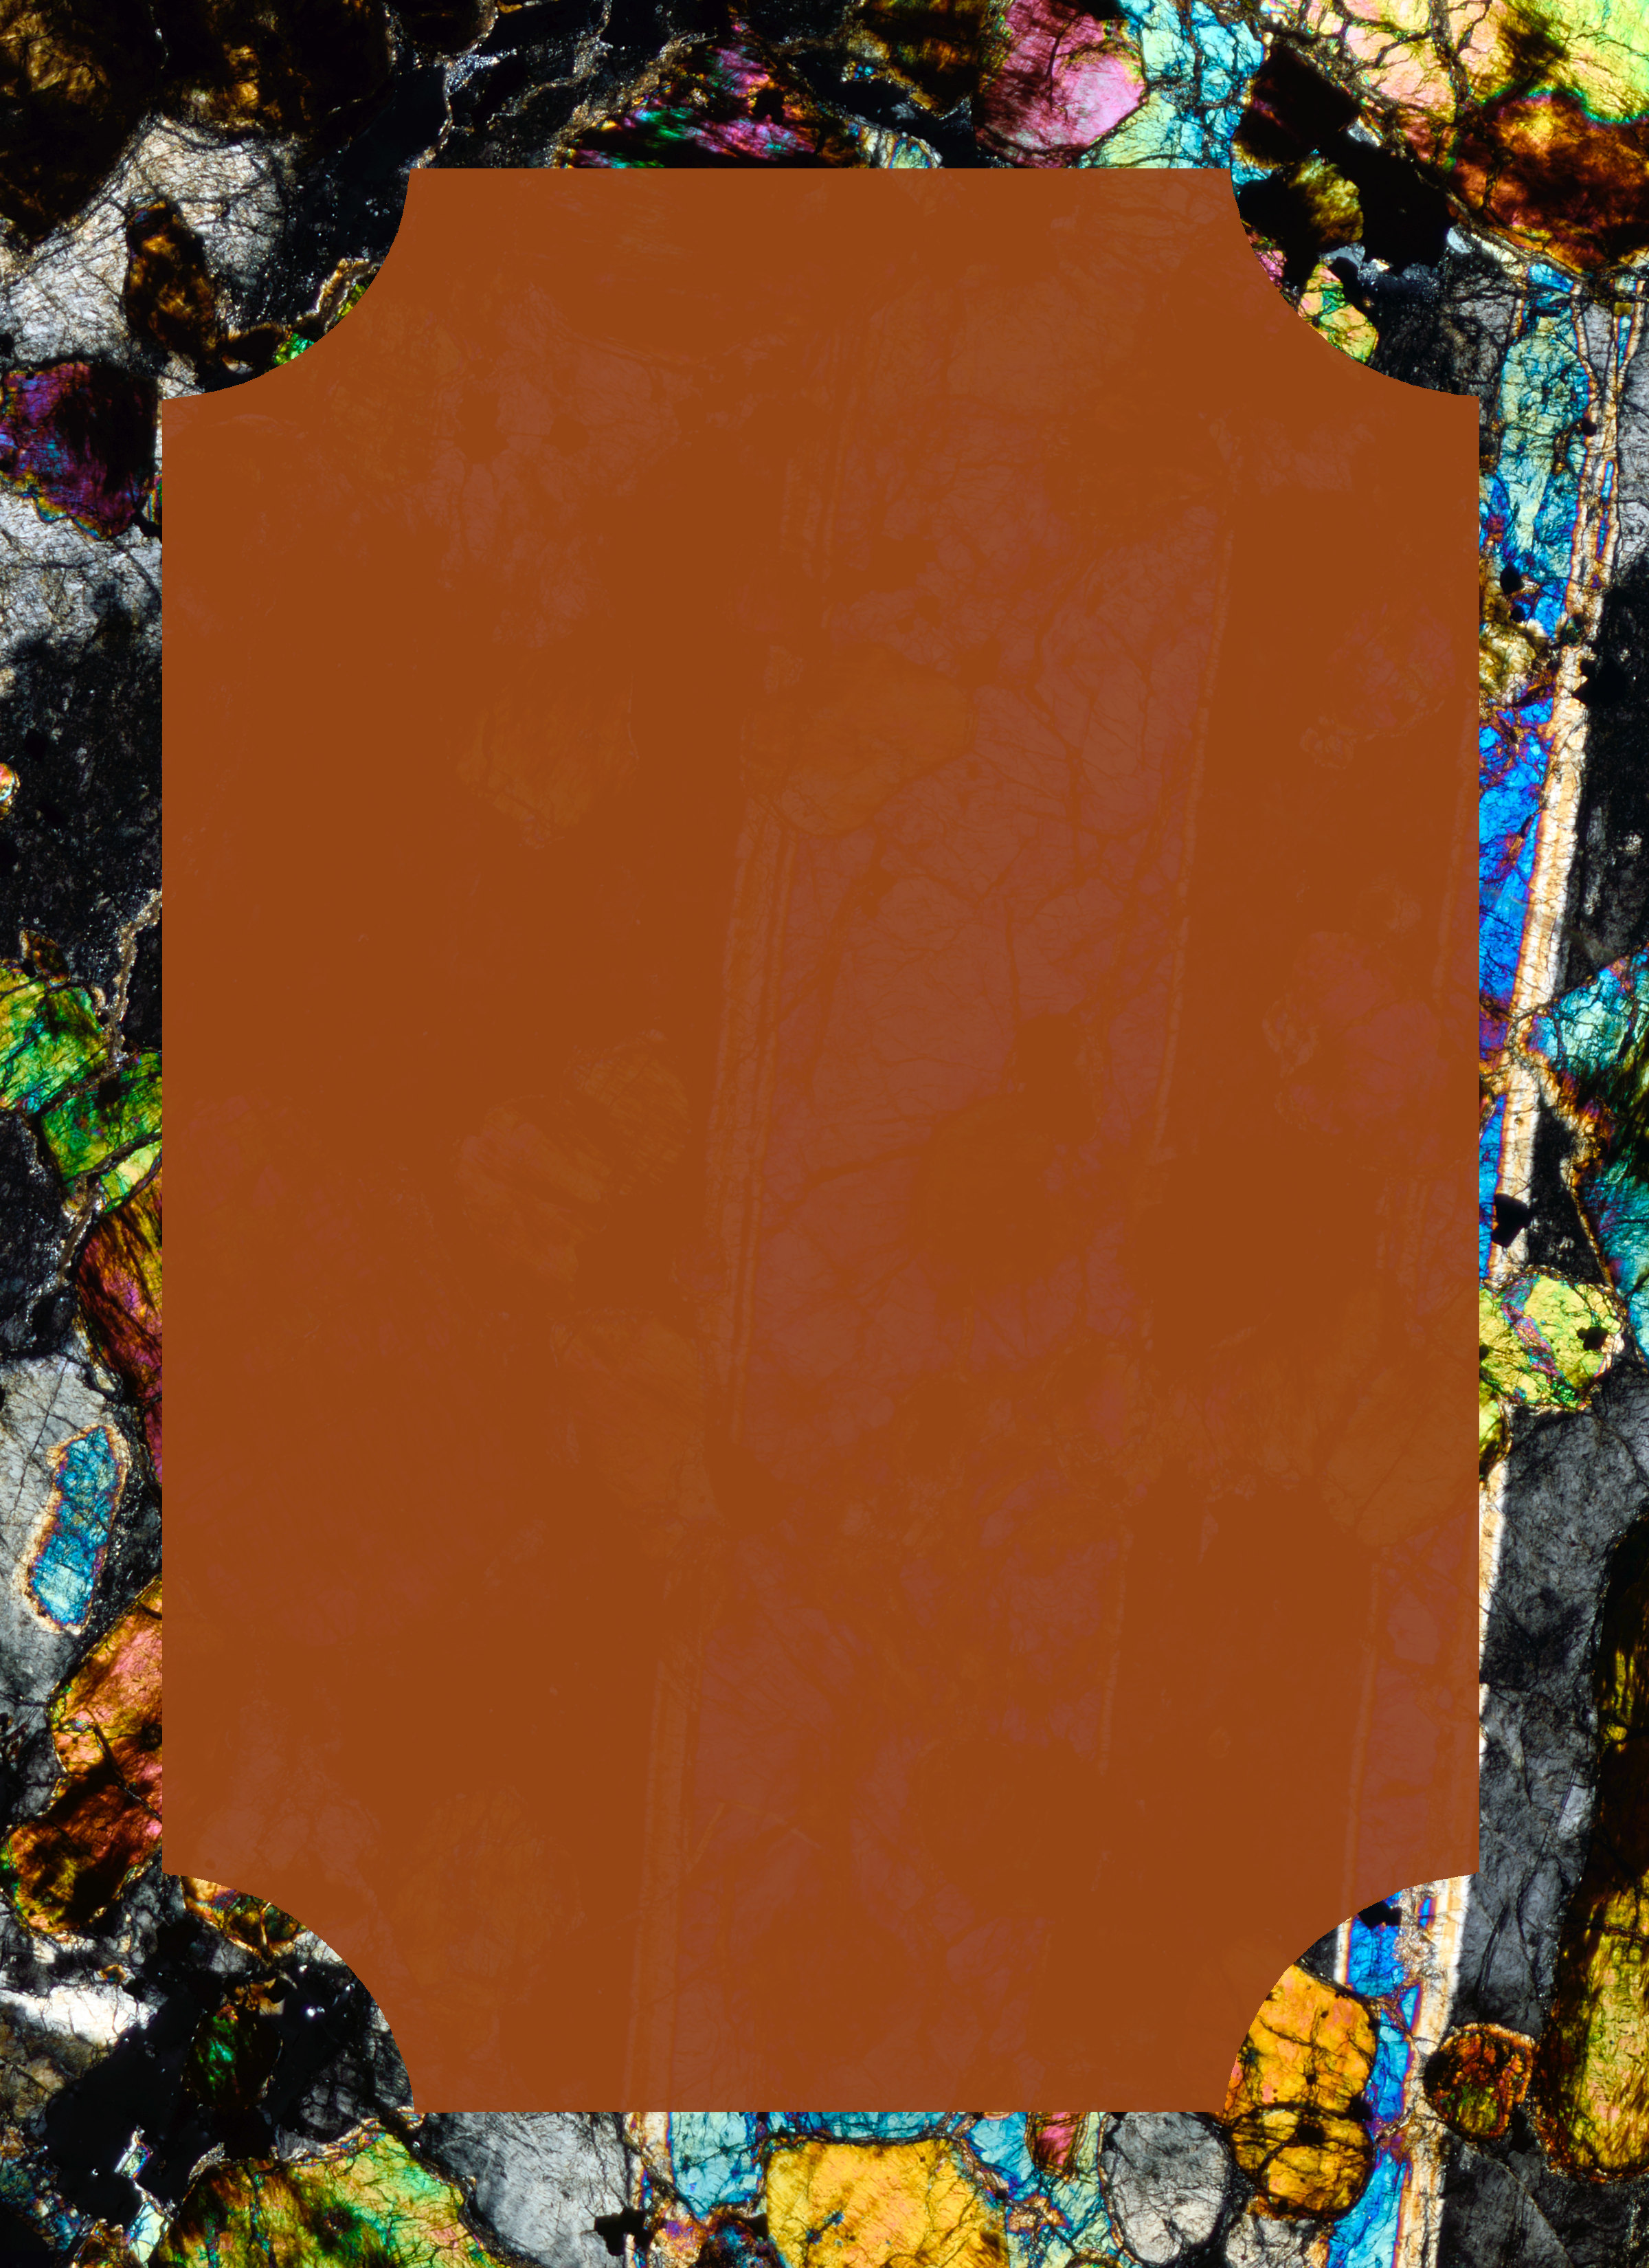
\includegraphics[width=\paperwidth,height=\paperheight]{mars2.jpeg}}
\begin{titlepage} % Suppresses headers and footers on the title page
	\centering % Centre everything on the title page
	%\scshape % Use small caps for all text on the title page

	%------------------------------------------------
	%	Title
	%------------------------------------------------

	\rule{\textwidth}{1.6pt}\vspace*{-\baselineskip}\vspace*{2pt} % Thick horizontal rule
	\rule{\textwidth}{0.4pt} % Thin horizontal rule
	
	\vspace{1\baselineskip} % Whitespace above the title
	
	{\Huge Περί Λίθων}
	
	\vspace{1\baselineskip} % Whitespace above the title

	\rule{\textwidth}{0.4pt}\vspace*{-\baselineskip}\vspace{3.2pt} % Thin horizontal rule
	\rule{\textwidth}{1.6pt} % Thick horizontal rule
	
	\vspace{1\baselineskip} % Whitespace after the title block
	
	%------------------------------------------------
	%	Subtitle
	%------------------------------------------------
	
	{\Large Θεόφραστος}
 
        \vspace{0.5\baselineskip}
	
	\vspace*{1\baselineskip} % Whitespace under the subtitle
	
        {\scshape \normalsize } % Subtitle or further description

	%------------------------------------------------
	%	Editor(s)
	%------------------------------------------------
        \vspace*{\fill}    

	\vspace{1\baselineskip}

	{\small\scshape Lipsiae 1862}
	
	{\small\scshape{Sumptibus et Typis B. G. Teubneri}}
	
	\vspace{0.5\baselineskip} % Whitespace after the title block

        {\scshape Internet Archive Online Edition}% Publication year}
    
	{\small CC Αναφορά-Μη Εμπορική Χρήση 4.0} % Publisher
\end{titlepage}
\setlength{\parskip}{1mm plus1mm minus1mm}
\clearpage
\large
%\tableofcontents
%\clearpage
1. Τῶν ἐν τῇ γῇ συνισταμένων τὰ μέν ἐστιν ὕδατος τὰ δὲ γῆς. ὕδατος μὲν τὰ μεταλλευόμενα καθάπερ ἄργυρος καὶ χρυσὸς καὶ τἆλλα, γῆς δὲ λίθος τε καὶ ὅσα λίθων εἴδη περιττότερα καὶ εἴ τινες δὴ τῆς γῆς αὐτῆς ἰδιώτεραι φύσεις εἰσὶν ἢ χρώμασιν ἢ λειότησιν ἢ πυκνότησιν ἢ ἄλλῃ τινὶ δυνάμει. περὶ μὲν οὖν τῶν μεταλλευομένων ἐν ἄλλοις τεθεώρηται · περὶ δὲ τούτων (λίθων?) νῦν λέγωμεν. ἅπαντα οὖν ταῦτα χρὴ νομίζειν ὡς ἁπλῶς εἰπεῖν ἐκ καθαρᾶς τινος συνεστᾶναι καὶ ὁμαλῆς ὕλης, εἴτε συρροῆς εἴτε διηθήσεώς τινος γενομένης, εἴτε ὡς ἀνωτέρω εἴρηται καὶ κατ' ἄλλον τρόπον ἐκκεκριμένης · τάχα γὰρ ἐνδέχεται τὰ μὲν οὕτως τὰ δ' ἐκείνως τὰ δ' ἄλλως. ἀφ' ὧν δὴ καὶ τὸ λεῖον καὶ τὸ πυκνὸν καὶ τὸ στιλπνὸν καὶ διαφανὲς καί τἆλλα τὰ τοιαῦτα ἔχουσι, καὶ ὅσῳ ἂν ὁμαλέστερον καὶ καθαρώτερον ἕκαστον ᾖ τοσούτῳ καὶ ταῦτα μᾶλλον ὑπάρχει. τὸ γὰρ ὅλον ὡς ἂν ἀκριβείας ἔχῃ τὰ κατὰ τὴν σύστασιν ἢ πῆξιν οὕτως ἀκολουθεῖ καὶ τὰ ἀπ' ἐκείνων. ἡ δὲ πῆξις τοῖς μὲν ἀπὸ θερμοῦ τοῖς δ' ἀπὸ ψυχροῦ γίνεται. κωλύει γὰρ ἴσως οὐδὲν ἔνια γένη λίθων ὑφ' ἑκατέρων συνίστασθαι τούτων. ἐπεὶ τά γε τῆς γῆς ἅπαντα δόξειεν ἂν ὑπὸ πυρός · ἐπείπερ τοῖς ἐναντίοις ἑκάστων ἡ πῆξις καὶ ἡ τῆξις. ἰδιότητες δὲ πλείους εἰσὶν ἐν τοῖς λίθοις · ἐν μὲν γὰρ τῇ γῇ χρώμασί τε καὶ γλισχρότητι καὶ λειότητι καὶ πυκνότητι καὶ τοῖς τοιούτοις αἱ πολλαὶ διαφοραὶ κατὰ δὲ τὰ ἄλλα σπάνιοι. τοῖς δὲ λίθοις αὗταί τε καὶ πρὸς ταύταις αἱ κατὰ τὰς δυνάμεις τοῦ τε ποιεῖν ἢ πάσχειν ἢ τοῦ μὴ πάσχειν. τηκτοὶ γὰρ οἱ δ' ἄτηκτοι, καὶ καυστοὶ οἱ δ' ἄκαυστοι, καὶ ἄλλα τούτοις ὅμοια. καὶ ἐν αὐτῇ τῇ καύσει καὶ πυρώσει πλείους ἔχοντες διαφοράς. ἔνιοι δὲ τοῖς χρώμασιν ἐξομοιοῦν λέγονται δυνάμενοι τὸ ὕδωρ ὥσπερ ἡ σμάραγδος, οἱ δ' ὅλως ἀπολιθοῦν τὰ τιθέμενα εἰς ἑαυτοὺς, ἕτεροι δὲ ὁλκήν τινα ποιεῖν, οἱ δὲ βασανίζειν τὸν χρυσὸν καὶ τὸν ἄργυρον ὥσπερ ἥ τε καλουμένη λίθος ἡρακλεία καὶ ἡ λυδή. θαυμασιωτάτη δὲ καὶ μεγίστη δύναμις, εἴπερ ἀληθὲς, ἡ τῶν τικτόντων · γνωριμωτέρα δὲ [τῶν] καὶ ἐν πλείοσι κατὰ τὰς ἐργασίας · γλυπτοὶ γὰρ ἔνιοι καὶ τορνευτοὶ καὶ πριστοὶ, τῶν δὲ οὐδὲ ὅλως ἅπτεται σιδήριον, ἐνίων δὲ κακῶς καὶ μόλις. εἰσὶ δὲ πλείους καὶ ἄλλαι παρὰ ταύτας διαφοραί. αἱ μὲν οὖν κατὰ τὰ χρώματα καὶ τὰς σκληρότητας καὶ μαλακότητας καὶ λειότητας καὶ τἆλλα τὰ τοιαῦτα διὰ τὸ περιττὸν πλείοσιν ὑπάρχουσι καὶ ἐνίοις γε κατὰ τόπον ὅλον. ἐξ ὧν δὴ καὶ διωνομασμέναι λιθοτομίαι Παρίων τε καὶ Πεντελικῶν καὶ Χίων τε καὶ Θηβαϊκῶν, καὶ ὡς ὁ περὶ Αἴγυπτον ἐν Θήβαις ἀλαβαστρίτης --- καὶ γὰρ οὗτος μέγας τέμνεται, --- καὶ ὁ τῷ ἐλέφαντι ὅμοιος ὁ χερνίτης καλούμενος, ἐν ᾗ πυέλῳ φασὶ καὶ Δαρεῖον κεῖσθαι. καὶ ὁ πόρος ὅμοιος τῷ χρώματι καὶ τῇ πυκνότητι τῷ παρίῳ τὴν δὲ κουφότητα μόνον ἔχων τοῦ πόρου, διὸ καὶ ἐν τοῖς σπουδαζομένοις οἰκήμασιν ὥσπερ διάζωμα τιθέασιν αὐτὸν οἱ Αἰγύπτιοι. καὶ μέλας αὐτόθι διαφανὴς ὅμοιος τῷ χίῳ, καὶ παρ' ἄλλοις δὲ ἕτεροι πλείους. αἱ μὲν οὖν τοιαῦται διαφοραὶ καθάπερ ἐλέχθη κοινότεραι πλείοσιν, αἱ δὲ κατὰ τὰς δυνάμεις τὰς προειρημένας οὐκέτι τόποις ὅλοις ὑπάρχουσιν οὐδὲ συνεχείαις, λίθων οὐδὲ μεγέθεσιν. ἔνιοι δὲ καὶ σπάνιοι πάμπαν εἰσὶ καὶ σμικροὶ καθάπερ ἥ τε σμάραγδος καὶ τὸ σάρδιον καὶ ὁ ἄνθραξ καὶ ἡ σάπφειρος καὶ σχεδὸν ... λόγον εἰς τὰ σφραγίδια γλυπτῶν. οἱ δὲ καὶ ἐν ἑτέροις εὑρίσκονται διακοπτομένοις. ὀλίγοι δὲ καί οἱ περὶ τὴν πύρωσιν καὶ καῦσιν, ὑπὲρ ὧν δὴ καὶ πρῶτον ἴσως λεκτέον τίνας καὶ πόσας ἔχουσι διαφοράς.

2. Κατὰ δὴ τὴν πύρωσιν οἱ μὲν τήκονται καὶ ῥέουσιν ὥσπερ οἱ μεταλλευτοί. ῥεῖ γὰρ ἅμα τῷ ἀργύρῳ καὶ τῷ χαλκῷ καὶ σιδήρῳ καὶ ἡ λίθος ἡ ἐκ τούτων, εἴτ' οὖν διὰ τὴν ὑγρότητα τῶν ἐνυπαρχόντων οἱ μυλίαι ῥέουσιν οἷς ἐπιτιθέασιν οἱ καίοντες. οἱ δὲ καὶ ὅλως λέγουσι πάντας τήκεσθαι πλὴν τοῦ μαρμάρου, τοῦτον δὲ κατακαίεσθαι καὶ κονίαν ἐξ αὐτοῦ γίνεσθαι. δόξειε δ' ἂν οὕτως ἐπὶ πλεῖον εἰρῆσθαι · πολλοὶ γὰρ οἱ ῥηγνύμενοι καὶ διαπηδῶντες ὡς ἀπομαχόμενοι τὴν πύρωσιν ὥσπερ [οὐδ'] ὁ κέραμος. ὃ καὶ κατὰ λόγον ἐστὶν, οἵτινες ἐξυγρασμένοι τυγχάνουσιν · τὸ γὰρ τηκτὸν ἔνικμον εἶναι δεῖ καὶ ὑγρότητ' ἔχειν πλείω. φασὶ δὲ καὶ τῶν ἡλιουμένων τοὺς μὲν ἀναξηραίνεσθαι τελείως ὥστ' ἀχρείους εἶναι μὴ καταβρεχθέντας πάλιν καὶ συνικμασθέντας τοὺς δὲ καὶ μαλακωτέρους καὶ διαθραύστους μᾶλλον. φανερὸν δὲ ὡς ἀμφοτέρων μὲν ἐξαιρεῖται τὴν ὑγρότητα, συμβαίνει δὲ τοὺς μὲν πυκνοὺς ἀποξηραινομένους σκληρύνεσθαι, τοὺς δὲ μανοὺς καὶ ὧν ἡ σύμφυσις τοιαύτη θραυστοὺς εἶναι καὶ τηκτούς. ἔνιοι δὲ τῶν θραυστῶν ἀνθρακοῦνται τῇ καύσει καὶ διαμένουσι πλείω χρόνον ὥσπερ οἱ περὶ Βίνας ἐν τῷ μετάλλῳ οὓς ὁ ποταμὸς καταφέρει · καίονται γὰρ ὅταν ἄνθρακες ἐπιτεθῶσι καὶ μέχρι τούτου ἄχρις ἂν φυσᾷ τις, εἶτ' ἀπομαραίνονται καὶ πάλιν καίονται, διὸ καὶ πολὺν χρόνον ἡ χρῆσις · ἡ δ' ὀσμὴ βαρεῖα σφόδρα καὶ δυσχερής. ὃν δὲ καλοῦσι σπῖνον, ὃς ἦν ἐν τοῖς (αὐτοῖς) μετάλλοις, οὗτος διακοπεὶς καὶ συντεθεὶς πρὸς ἑαυτὸν ἐν τῷ ἡλίῳ τιθέμενος καίεται, καὶ μᾶλλον ἐὰν ἐπιψεκάσῃ καὶ περιράνῃ τις. ὁ δὲ λιπαραῖος ἐκφοροῦταί τε τῇ καύσει καὶ γίνεται κισσηροειδὴς ὥσθ' ἅμα τήν τε χρόαν μεταβάλλειν καὶ τὴν πυκνότητα · μέλας τε γὰρ καὶ λεῖός ἐστι καὶ πυκνὸς ἄκαυστος ὤν. γίνεται δὲ οὗτος ἐν τῇ κισσήρει διειλημμένος ἄλλοθι καὶ ἄλλοθι καθάπερ ἐν κυττάρῳ καὶ οὐ συνεχὴς, ὥσπερ καὶ ἐν Μήλῳ φασὶ τὴν κίσσηριν ἐν ἄλλῳ τινὶ λίθῳ γίνεσθαι. καὶ ἐκεῖνος μὲν τούτῳ ὥσπερ ἀντιπεπονθώς · πλὴν ὁ λίθος οὗτος οὐχ ὅμοιος τῷ λιπαραίῳ. ἐκφοροῦται δὲ καὶ ὁ ἐν Τετράδι τῆς Σικελίας γινόμενος · τοῦτο δὲ τὸ χωρίον ἐστὶ κατὰ Λιπάραν, ὁ δὲ λίθος ἐν τῇ ἄκρᾳ τῇ Ἐρινεάδι καλουμένῃ πολὺς ὁμοίως τῷ ἐν Βίναις καιόμενος ὀσμὴν ἀφίησιν ἀσφάλτου, τὸ δ' ἐκ τῆς κατακαύσεως ὅμοιον γίνεται γῇ κεκαυμένῃ. οὓς δὲ καλοῦσιν εὐθὺς ἄνθρακας τῶν ὀρυττομένων διὰ τὴν χρείαν εἰσὶ γεώδεις, ἐκκαίονται δὲ καὶ πυροῦνται καθάπερ οἱ ἄνθρακες. εἰσὶ δὲ περί τε τὴν Λιγυστικὴν ὅπου καὶ τὸ ἤλεκτρον, καὶ ἐν τῇ Ἠλείᾳ βαδιζόντων Ὀλυμπίαζε τὴν δι' ὄρους, οἷς καὶ οἱ χαλκεῖς χρῶνται. εὑρέθη δέ ποτε ἐν τοῖς Σκαπτησύλης μετάλλοις λίθος ὃς τῇ μὲν ὄψει παρόμοιος ὢν ξύλῳ σαπρῷ, ὅτε δ' ἐπιχέοιτό τις ἔλαιον καίεται, καὶ ὅτ' ἐκκαυθείη τότε παύεται καὶ αὐτὸς ὥσπερ ἀπαθὴς ὤν. τῶν μὲν οὖν καιομένων σχεδὸν αὗται διαφοραί.

3. Ἄλλο δέ τι γένος ἐστὶ λίθων ὥσπερ ἐξ ἐναντίων πεφυκὸς, ἄκαυστον ὅλως, ἄνθραξ καλούμενος, ἐξ οὗ καὶ τὰ σφραγίδια γλύφουσιν, ἐρυθρὸν μὲν τῷ χρώματι, πρὸς δὲ τὸν ἥλιον τιθέμενον ἄνθρακος καιομένου ποιεῖ χρόαν. τιμιώτατον δ' ὡς εἰπεῖν · μικρὸν γὰρ σφόδρα τετταράκοντα χρυσῶν. ἄγεται δὲ οὗτος ἐκ Καρχηδόνος καὶ Μασσαλίας. οὐ καίεται δὲ ὁ περὶ Μίλητον γωνιοειδὴς ὢν ἐν ᾧπερ καὶ τὰ ἑξάγωνα. καλοῦσι δ' ἄνθρακα καὶ τοῦτον, ὃ καὶ θαυμαστόν ἐστιν · ὅμοιον γὰρ τρόπον τινὰ καὶ τὸ τοῦ ἀδάμαντος · οὐ γὰρ οὐδ' ὥσπερ ἡ κίσσηρις καὶ τέφρα δόξειεν ἂν διὰ τὸ μηδὲν ἔχειν ὑγρόν · ταῦτα γὰρ ἄκαυστα καὶ ἀπύρωτα διὰ τὸ ἐξῃρῆσθαι τὸ ὑγρόν · ἐπεὶ καὶ τὸ ὅλον ἡ κίσσηρις ἐκ κατακαύσεως δοκεῖ τισι γίνεσθαι, πλὴν τῆς ἐκ τοῦ ἀφροῦ τῆς θαλάσσης συνισταμένης. λαμβάνουσι δὲ τὴν πίστιν διὰ τῆς αἰσθήσεως ἔκ τε τῶν περὶ τοὺς κρατῆρας γινομένων καὶ ἐκ τῆς διαβάρου λίθου τῆς φλογουμένης * οὐ κισσηροῦται. μαρτυρεῖν δὲ καὶ οἱ τόποι δοκοῦσιν ἐν οἷς ἡ γένεσις · καὶ γὰρ ἐν τοῖς * μάλιστα καὶ ἡ κίσσηρις. τάχα δὲ ἡ μὲν οὕτως αἱ δ' ἄλλως καὶ πλείους τρόποι τῆς γενέσεως. ἡ γὰρ ἐν Νισύρῳ καθάπερ ἐξ ἄμμου τινὸς ἔοικε συγκεῖσθαι. σημεῖον δὲ λαμβάνουσιν ὅτι τῶν εὑρισκομένων ἔνιαι διαθρύπτονται ἐν ταῖς χερσὶν ὥσπερ εἰς ἄμμον διὰ τὸ μήπω συνεστάναι μηδὲ συμπεπηγέναι. εὑρίσκουσι δ' ἀθρόας κατὰ μικρὰ χειροπληθεῖς ὅσον πολλὰς ἢ μικρῷ μείζους ὅταν ἀπαμήσωνται τἄνω · ἐλαφρὰ δὲ σφόδρα ἡ ἄμμος. ἡ δ' αὖ καὶ ἐν Μήλῳ πᾶσα μὲν * ἔνια δ' αὖ ἐν λίθῳ τινὶ ἑτέρῳ γίνεται καθάπερ ἐλέχθη πρότερον. διαφορὰς δ' ἔχουσι πρὸς ἀλλήλας καὶ χρώματι καὶ πυκνότητι καὶ βάρει · χρώματι μὲν ὅτι μέλαινα ἐκ τοῦ ῤύακος τοῦ ἐν Σικελίᾳ · πυκνότητι δὲ καὶ βάρει αὕτη τε καὶ μαλώδης. γίνεται γάρ τις καὶ τοιαύτη κίσσηρις καὶ βάρος ἔχει καὶ πυκνότητα καὶ ἐν τῇ χρήσει πολυτιμότερον τῆς ἑτέρας. τμητικὴ δὲ καὶ ἡ ἐκ τοῦ ῥύακος μᾶλλον τῆς κούφης καὶ λευκῆς, τμητικωτάτη δ' ἐκ τῆς θαλάσσης αὐτῆς. καὶ περὶ μὲν κισσηρίδος ἐπὶ τοσοῦτον εἰρήσθω. περὶ δὲ τῶν πυρουμένων καὶ τῶν ἀπυρώτων λίθων ἀφ' ὧν καὶ εἰς τοῦτο ἐξέβημεν ἐν ἄλλοις θεωρητέον τὰς αἰτίας.

4. Τῶν δὲ λίθων καὶ ἄλλαι (διάφοροι) τυγχάνουσιν ἐξ ὧν καὶ τὰ σφραγίδια γλύφουσιν. αἱ μὲν τῇ ὄψει μόνον οἷον τὸ σάρδιον καὶ ἡ ἴασπις καὶ σάπφειρος · αὕτη δ' ἐστὶν ὥσπερ χρυσόπαστος. ἡ δὲ σμάραγδος καὶ δυνάμεις τινὰς ἔχει · τοῦ τε γὰρ ὕδατος ὥσπερ εἴπομεν ἐξομοιοῦται τὴν χρόαν ἑαυτῇ, μεταρία μὲν οὖσα ἐλάττονος, ἡ δὲ μεγίστη παντὸς, ἡ δὲ χειρίστη τοῦ καθ' αὑτὴν μόνον. καὶ πρὸς τὰ ὄμματα ἀγαθὴ, διὸ καὶ τὰ σφραγίδια φοροῦσιν ἐξ αὐτῆς ὥστε βλέπειν · ἔστι δὲ σπανία καὶ τὸ μέγεθος οὐ μεγάλη, πλὴν εἰ πιστεύειν ταῖς ἀναγραφαῖς δεῖ ὑπὲρ τῶν βασιλέων τῶν αἰγυπτίων · ἐκείνοις γάρ φασι κομισθῆναί ποτ' ἐν δώροις παρὰ τοῦ Βαβυλωνίων βασιλέως μῆκος μὲν τετράπηχυν πλάτος δὲ τρίπηχυν. ἀνακεῖσθαι δὲ καὶ ἐν τῷ τοῦ Διὸς ὀβελίσκῳ σμαράγδους τέτταρας, μῆκος μὲν τετταράκοντα πηχῶν, εὖρος δὲ τῇ μὲν τέτταρας τῇ δὲ δύο. ταῦτα μὲν οὖν ὅτι κατὰ τὴν ἐκείνων γραφήν. τῶν δὲ βακτριανῶν καλουμένων ὑπὸ πολλῶν ἡ ἐν Τύρῳ μεγίστη. στήλη γάρ ἐστιν εὐμεγέθης ἐν τῷ τοῦ Ἡρακλέους ἱερῷ · εἰ μὴ ἄρα ψευδὴς σμάραγδος, καὶ γὰρ τοιαύτη γίνεταί τις φύσις. γίνεται δὲ ἐν τοῖς ἐν ἐφικτῷ καὶ γνωρίμοις τόποις διτταχοῦ μάλιστα περί τε Κύπρον ἐν τοῖς χαλκορυχείοις καὶ ἐν τῇ νήσῳ τῇ ἐπικειμένῃ Χαλκηδόνι. καὶ ἰδιωτέρους εὑρίσκουσιν ἐν ταύτῃ · μεταλλεύεται γὰρ ὥσπερ τἆλλα καὶ ἡ φύσις κατὰ ῥάβδους ἐποίησεν ἐν Κύπρῳ αὐτὴν καθ' αὑτὴν πολλάς. εὑρίσκονται δὲ σπάνιαι μέγεθος ἔχουσαι σφραγίδος ἀλλ' ἐλάττους αἱ πολλαὶ, διὸ καὶ πρὸς τὴν κόλλησιν αὐτῇ χρῶνται τοῦ χρυσίου · κολλᾷ γὰρ ὥσπερ ἡ χρυσοκόλλα. καὶ ἔνιοί γε δὴ καὶ ὑπολαμβάνουσι τὴν αὐτὴν φύσιν εἶναι · καὶ γὰρ τὴν χρόαν παρόμοιαι τυγχάνουσιν. ἀλλ' ἡ μὲν χρυσοκόλλα δαψιλὴς καὶ ἐν τοῖς χρυσείοις καὶ ἔτι μᾶλλον ἐν τοῖς χαλκορυχείοις ὥσπερ ἐν τοῖς περὶ τοὺς * τόπους. ἡ δὲ σμάραγδος σπανία καθάπερ εἴρηται · δοκεῖ γὰρ ἐκ τῆς ἰάσπιδος γίνεσθαι. φασὶ γὰρ εὑρεθῆναί ποτε ἐν Κύπρῳ λίθον ἧς τὸ μὲν ἥμισυ σμάραγδος ἦν τὸ ἥμισυ δὲ ἴασπις ὡς οὔπω μεταβεβληκυίας ἀπὸ τοῦ ὕδατος. ἔστι δέ τις αὐτῆς ἐργασία πρὸς τὸ λαμπρόν · ἀργὴ γὰρ οὖσα οὐ λαμπρά.

5. Αὕτη τε δὴ περιττὴ τῇ δυνάμει καὶ τὸ λυγγούριον · καὶ γὰρ ἐκ τούτου γλύφεται τὰ σφραγίδια καὶ ἔστι στερεωτάτη καθάπερ λίθος · ἕλκει γὰρ ὥσπερ τὸ ἤλεκτρον, οἱ δέ φασιν οὐ μόνον κάρφη καὶ ξύλον (φύλλα?) ἀλλὰ καὶ χαλκὸν καὶ σίδηρον ἐὰν ᾖ λεπτὸς, ὥσπερ καὶ Διοκλῆς ἔλεγεν. ἔστι δὲ διαφανές τε σφόδρα καὶ ψυχρόν. βέλτιον δὲ τὸ τῶν ἀγρίων ἢ τὸ τῶν ἡμέρων καὶ τὸ τῶν ἀρρένων ἢ τὸ τῶν θηλειῶν ὡς καὶ τῆς τροφῆς διαφερούσης, καὶ τοῦ πονεῖν ἢ μὴ πονεῖν. καὶ τῆς τοῦ σώματος ὅλως φύσεως, ᾗ τὸ μὲν ξηρότερον τὸ δ' ὑγρότερον. εὑρίσκουσι δ' ἀνορύττοντες οἱ ἔμπειροι · κατακρύπτεται γὰρ καὶ ἐπαμᾶται γῆν ὅταν οὐρήσῃ. γίνεται δὲ καὶ κατεργασία τις αὐτοῦ πλείων. ἐπεὶ δὲ καὶ τὸ ἤλεκτρον λίθος, τὸ γὰρ ὀρυκτὸν ὃ περὶ Λιγυστικὴν, καὶ τούτῳ ἂν ἡ τοῦ ἕλκειν δύναμις ἀκολουθοίη. μάλιστα δ' ἐπίδηλος καὶ φανερωτάτη ἡ τὸν σίδηρον ἄγουσα. γίνεται δὲ καὶ αὕτη σπανία καὶ ὀλιγαχοῦ. καὶ αὕτη μὲν δὴ συναριθμείσθω τὴν δύναμιν ὁμοίαν ἔχειν. ἐξ ὧν δὲ τὰ σφραγίδια ποιεῖται καὶ ἄλλαι πλείους εἰσὶν, οἷον ἥ θ' ὑαλοείδης ἣ καὶ ἔμφασιν ποιεῖ καὶ διάφασιν, καὶ τὸ ἀνθράκιον, καὶ ἡ ὄμφαξ · ἔτι δὲ καὶ ἡ κρύσταλλος καὶ τὸ ἀμέθυσον, ἄμφω δὲ διαφανὴ εὑρίσκονται δὲ καὶ αὗται καὶ τὸ σάρδιον διακοπτομένων τινῶν πετρῶν. καὶ ἄλλαι δὲ ὡς προείρηται πρότερον διαφορὰς ἔχουσαι καὶ συνώνυμοι πρὸς ἀλλήλας. τοῦ γὰρ σαρδίου τὸ μὲν διαφανὲς ἐρυθρότερον δὲ καλεῖται θῆλυ, τὸ δὲ διαφανὲς μὲν μελάντερον δὲ [καὶ] ἄρσεν. καὶ τὰ λυγγούρια δὲ ὡσαύτως ὧν τὸ θῆλυ διαφανέστερον καὶ ξανθότερον. καλεῖται δὲ καὶ κύανος ὁ μὲν ἄρρην ὁ δὲ θῆλυς · μελάντερος δὲ ὁ ἄρρην. τὸ δ' ὀνύχιον μικτὸν λευκῷ καὶ φαιῷ παρ' ἄλληλα. τὸ δ' ἀμέθυσον οἰνωπὸν τῇ χρόᾳ. καλὸς δὲ λίθος καὶ ὁ ἀχάτης ὁ ἀπὸ τοῦ Ἀχάτου ποταμοῦ τοῦ ἐν Σικελίᾳ καὶ πωλεῖται τίμιος. ἐν Λαμψάκῳ δέ ποτ' ἐν τοῖς χρυσίοις εὑρέθἡ θαυμαστὴ λίθος ἐξ ἧς ἀνενεχθείσης πρὸς * στιρὰν (Ἄστυρα Schn.) σφραγίδιον γλυφθὲν ἀνεπέμφθη (Ἀλεξάνδρῳ Plin.) βασιλεῖ διὰ τὸ περιττόν.

6. Καὶ αὗται μὲν ἅμα τῷ καλῷ καὶ τὸ σπάνιον ἔχουσιν. αἱ δὲ δὴ ἐκ τῆς Ἑλλάδος εὐτελέστεραι, οἷον τὸ ἀνθράκιον τὸ ἐξ Ὀρχομενοῦ τῆς Ἀρκαδίας. ἔστι δὲ οὗτος μελάντερος τοῦ Χίου · κάτοπτρα δὲ ἐξ αὐτοῦ ποιοῦσι · καὶ ὁ τροιζήνιος · οὗτος δὲ ποικίλος τὰ μὲν φοινικοῖς τὰ δὲ λευκοῖς χρώμασι. ποικίλος δὲ καὶ ὁ κορίνθιος τοῖς αὐτοῖς χρώμασι πλὴν ὅτι χλωροειδέστερος. τὸ δὲ ὅλον πολλοὶ τυγχάνουσιν οἱ τοιοῦτοι ἀλλ' οἱ περιττοὶ σπάνιοι καὶ ἐξ ὀλίγων τόπων οἷον ἔκ τε Καρχηδόνος καὶ ἐκ τῶν περὶ Μασσαλίαν καὶ ἐξ Αἰγύπτου κατὰ τοὺς Καταδούπους καὶ Συήνης πρὸς Ἐλεφαντίνῃ πόλει καὶ ἐκ τῆς Ψεφὼ καλουμένης χώρας. καὶ ἐν Κύπρῳ ἥ τε σμάραγδος καὶ ἡ ἴασπις. οἷς δὲ εἰς τὰ λιθοκόλλητα χρῶνται ἐκ τῆς Βακτριανῆς εἰσὶ πρὸς τῇ ἐρήμῳ. συλλέγουσι δ' αὐτοὺς ὑπὸ ἐτησίας ἱππεῖς ἐξιόντες · τότε γὰρ ἐμφανεῖς γίνονται κινουμένης τῆς ἄμμου διὰ τὸ μέγεθος τῶν πνευμάτων. εἰσὶ δὲ μικροὶ καὶ οὐ μεγάλοι. τῶν σπουδαζομένων δὲ λίθων ἐστὶ καὶ ὁ μαργαρίτης καλούμενος, διαφανὴς μὲν τῇ φύσει, ποιοῦσι δ' ἐξ αὐτοῦ τοὺς πολυτελεῖς ὅρμους. γίνεται δὲ ἐν ὀστρείῳ τινὶ παραπλησίῳ ταῖς πίνναις, (πλὴν ἐλάττονι · μέγεθος δὲ ἡλίκος ἰχθύος ὀφθαλμὸς εὐμεγέθης · Athen.) φέρει δὲ ἥ τε Ἰνδικὴ χώρα καὶ νῆσοί τινες τῶν ἐν τῇ ἐρυθρᾷ. τὸ μὲν οὖν περιττὸν σχεδὸν ἐν ταύταις. εἰσὶ δὲ καὶ ἄλλαι τινὲς, οἷον ὁ ἐλέφας ὁ ὀρυκτὸς ποικίλος μέλανι καὶ λευκῷ. καὶ ἣν καλοῦσι σάπφειρον · αὕτη γὰρ μέλαινα οὐκ ἄγαν πόρρω τοῦ κυάνου τοῦ ἄρρενος καὶ πρασίτις · αὕτη δὲ ἰώδης τῇ χρόᾳ. πυκνὴ δὲ καὶ αἱματίτις · αὕτη δ' αὐχμώδης καὶ κατὰ τοὔνομα ὡς αἵματος ξηροῦ πεπηγότος. ἄλλη δὲ ἡ καλουμένη ξανθὴ, οὐ ξανθὴ μὲν τὴν χρόαν ἔκλευκος δὲ μάλλον, ὃ καλοῦσι χρῶμα οἱ Δωριεῖς ξανθόν. τὸ γὰρ κουράλιον, καὶ γὰρ τοῦθ' ὥσπερ λίθος, τῇ χρόᾳ μὲν ἐρυθρὸν, περιφερὲς δ' ὡς ῥίζα · φύεται δ' ἐν τῇ θαλάττῃ. τρόπον δέ τινα οὐ πόρρω τούτου τῇ φύσει καὶ ὁ ἰνδικὸς κάλαμος ἀπολελιθωμένος. ταῦτα μὲν οὖν ἄλλης σκέψεως.

7. Τῶν δὲ λίθων πολλαί τινες αἱ φύσεις καὶ τῶν μεταλλευομένων. ἔνιαι γὰρ ἅμα χρυσὸν ἔχουσι καὶ ἄργυρον, προφανῆ δὲ μόνον ἄργυρον · βαρύτεραι δὲ αὗται πολὺ καὶ τῇ ῥοπῇ καὶ τῇ ὀσμῇ. καὶ κύανος αὐτοφυὴς ἔχων ἐν ἑαυτῷ χρυσοκόλλαν. ἄλλη δὲ λίθος ὁμοία τὴν χρόαν τοῖς ἄνθραξι · βάρος δὲ ἔχουσι. τὸ δὲ ὅλον ἐν τοῖς μετάλλοις πλεῖσται καὶ ἰδιώταται φύσεις εὑρίσκονται τῶν τοιούτων, ὧν τὰ μέν εἰσι γῆς καθάπερ ὦχρα καὶ μίλτος, τὰ δὲ οἷον ἄμμου καθάπερ χρυσοκόλλα καὶ κύανος, τὰ δὲ κονίας οἷον σανδαράκη καὶ ἀρρενικὸν καὶ ὅσα ὅμοια τούτοις. καὶ τῶν μὲν τοιούτων πλείους ἄν τις λάβοι τὰς ἰδιότητας. ἔνιαι δὲ λίθοι καὶ τὰς τοιαύτας ἔχουσι δυνάμεις εἰς τὸ μὴ πάσχειν, ὥσπερ εἴπομεν, οἷον τὸ μὴ γλύφεσθαι σιδηρίοις ἀλλὰ λίθοις ἑτέροις. ὅλως μὲν ἡ κατὰ τὰς ἐργασίας καὶ τῶν μειζόνων λίθων πολλὴ διαφορά. πριστοὶ γὰρ, οἱ δὲ γλυπτοὶ, καθάπερ ἐλέχθη, καὶ τορνευτοὶ τυγχάνουσι, καθάπερ καὶ ἡ μαγνῆτις αὕτη λίθος ἡ καὶ ὄψει περιττὸν ἔχουσα, καὶ ἧς γε δή τινες θαυμάζουσι τὴν ὁμοίωσιν τῷ ἀργύρῳ μηδαμῶς οὔσης συγγενοῦς. πλείους δ' εἰσὶν οἱ δεχόμενοι πάσας τὰς ἐργασίας. ἐπεὶ καὶ ἐν Σίφνῳ τοιοῦτός τίς ἐστιν ὀρυκτὸς ὡς τρία στάδια ἀπὸ θαλάττης, στρογγύλος καὶ βωλώδης, καὶ τορνεύεται καὶ γλύφεται διὰ τὸ μαλακόν · ὅταν δὲ πυρωθῇ καὶ ἀποβαφῇ [τῷ] ἐλαίῳ, μέλας τε σφόδρα γίνεται καὶ σκληρός. ποιοῦσι δ' ἐξ αὐτοῦ σκεύη τὰ ἐπιτράπεζα. οἱ μὲν (οὖν) τοιοῦτοι πάντες προσδέχονται τὴν τοῦ σιδήρου δύναμιν · ἔνιοι δὲ λίθοις ἄλλοις γλύφονται, σιδήροις δ' οὐ δύνανται καθάπερ εἴπομεν. οἱ δὲ σιδήροις μὲν ἀμβλυτέροις δέ · καὶ εἰσὶν ... παραπλησίως δὲ κάτω (ἄτοπον?) τὰ ... μὴ τέμνεσθαι ... σιδήρῳ καίτοι καὶ στερεὸν ἕτε ... ἰσχυρότερα τέμνει, καὶ σίδηρος λίθου σκληρότερος ὤν. ἄτοπον δὲ κἀκεῖνο φαίνεται διότι ἡ μὲν ἀκόνη κατεσθίει τὸν σίδηρον, ὁ δὲ σίδηρος ταύτην μὲν δύναται διαιρεῖν καὶ ῥυθμίζειν, ἐξ ἧς δὲ αἱ σφραγίδες οὔ. καὶ πάλιν ὁ λίθος ᾧ γλύφουσι τὰς σφραγίδας ἐκ τούτου ἐστὶν ἐξ οὗπερ αἱ ἀκόναι, ἢ ἐξ ὁμοίου τούτῳ · ἄγεται δὲ ἡ (ἀρίστη) ἐξ Ἀρμενίας. θαυμαστὴ δὲ φύσις καὶ τῆς βασανιζούσης τὸν χρυσόν · δοκεῖ γὰρ δὴ τὴν αὐτὴν ἔχειν τῷ πυρὶ δύναμιν · καὶ γὰρ ἐκεῖνο δοκιμάζει. διὸ καὶ ἀποροῦσί τινες οὐκ ἄγαν οἰκείως ἀποροῦντες. οὐ γὰρ τὸν αὐτὸν τρόπον δοκιμάζει, ἀλλὰ τὸ μὲν πῦρ τῷ τὰ χρώματα μεταβάλλειν καὶ ἀλλοιοῦν ὁ δὲ λίθος τῇ παρατρίψει · δύναται γὰρ ὡς ἔοικεν ἐκλαμβάνειν τὴν ἑκάστου φύσιν. εὑρῆσθαι δέ φασι νῦν ἀμείνω πολὺ τῆς πρότερον ὥστε μὴ μόνον τὸν ἐκ τῆς καθάρσεως ἀλλὰ καὶ τὸν κατάχαλκον χρυσὸν καὶ ἄργυρον γνωρίζειν καὶ πόσον εἰς τὸν στατῆρα μέμικται. σημεῖα δ' ἐστὶν αὐτοῖς ἀπὸ τοῦ ἐλαχίστου · ἐλάχιστον δὲ γίνεται κριθὴ, εἶτα κόλλυβος, εἶτα τεταρτημόριον ἢ ἡμιώβολος, ἐξ ὧν γνωρίζουσι τὸ καθῆκον. εὑρίσκονται δὲ τοιαῦται πᾶσαι ἐν τῷ ποταμῷ Τμώλῳ. λεία δ' ἡ φύσις αὐτῶν καὶ ψηφοειδὴς, πλατεῖα, οὐ στρογγύλη. μέγεθος δὲ ὅσον διπλασία τῆς μεγίστης ψήφου. διαφέρει δ' αὐτῆς πρὸς τὴν δοκιμασίαν τὰ ἄνω πρὸς τὸν ἥλιον ἢ τὰ κάτω καὶ βέλτιον δοκιμάζει τὰ ἄνω · τοῦτο δὲ διότι ξηρότερα τὰ ἄνω · κωλύει γὰρ ἡ ὑγρότης εἰς τὸ ἐκλαμβάνειν · ἐπειδὴ καὶ ἐν τοῖς καύμασι δοκιμάζει χεῖρον · ἀνίησι γάρ τινα νοτίδα ἐξ αὐτὴς δι' ἣν ἀπολισθαίνει. συμβαίνει δὲ τοῦτο καὶ ἄλλοις τῶν λίθων, καὶ ἐξ ὧν τὰ ἀγάλματα ποιοῦσιν, ὃ καὶ σημεῖον ὑπολαμβάνουσιν ἴδιόν τι τοῦ ἕδους.

8. Αἱ μὲν οὖν τῶν λίθων διαφοραὶ καὶ δυνάμεις εἰσὶν ἐν τούτοις. αἱ δὲ τῆς γῆς ἐλάττονες μὲν ἰδιώτεραι δέ. τὸ μὲν γὰρ τήκεσθαι καὶ μαλάττεσθαι καὶ πάλιν ἀποσκληρύνεσθαι καὶ ταύτῃ συμβαίνει. τήκεται μὲν γὰρ * τοῖς χυτοῖς καὶ ὀρυκτοῖς ὥσπερ καὶ ὁ λίθος · μαλάττεται δὲ, λίθους τε ποιοῦσιν, ὧν τάς τε ποικίλας καὶ τὰς ἄλλας συντιθεμένας ... ἁπάσας γὰρ πυροῦντες καὶ μαλάττοντες ποιοῦσιν. εἰ δὲ καὶ ὁ ὕελος ἐκ τῆς ὑελίτιδος ὥς τινές φασι, καὶ αὕτη πυκνώσει γίνεται. ἰδιωτάτη δὲ ἡ τῷ χαλκῷ μιγνυμένη · πρὸς γὰρ τῷ τήκεσθαι καὶ μίγνυσθαι καὶ δύναμιν ἔχει περιττὴν ὥστε τῷ κάλλει τῆς χρόας ποιεῖν διαφοράν. περὶ δὲ Κιλικίαν ἐστί τις ἣ ἕψεται γῆ καὶ γίνεται γλισχρά · ταύτῃ δ' ἀλείφουσι τὰς ἀμπέλους ἀντὶ ἰξοῦ πρὸς τοὺς ἶπας. εἴη δ' ἂν λαμβάνειν καὶ ταύτας τὰς διαφορὰς, ὅσαι πρὸς τὴν ἀπολίθωσιν εὐφυεῖς · ἐπεὶ αἵ γε τῶν τόπων ποιοῦσαι χυμοὺς διαφόρους ἀλλήλων (ἰδίαν) τιν' ἔχουσι φύσιν, ὥσπερ καὶ αἱ τοὺς τῶν φυτῶν. ἀλλὰ μᾶλλον ἄν τις (αὐ)τὰς τοῖς χρώμασι διαριθμήσειεν οἷσπερ καὶ οἱ γραφεῖς χρώνται. καὶ γὰρ ἡ γένεσις τούτων, ὥσπερ ἐξ ἀρχῆς εἴπομεν, ἤτοι συρροῆς τινὸς ἢ διηθήσεως γινομένης. καὶ ἔνιά γε δὴ φαίνεται πεπυρωμένα καὶ οἷον κατακεκαυμένα οἷον καὶ ἡ σανδαράκη καὶ τὸ ἀρρενικὸν καὶ τὰ ἄλλα τὰ τοιαῦτα. πάντα δ' ὡς ἁπλῶς εἰπεῖν ἀπὸ τῆς ἀναθυμιάσεως ταῦτα τῆς ξηρᾶς καὶ καπνώδους. εὑρίσκεται δὴ πάντα ἐν τοῖς μετάλλοις τοῖς ἀργυρείοις τε καὶ χρυσείοις, ἔνια δὲ καὶ ἐν τοῖς χαλκορυχείοις, οἷον ἀρρενικὸν, σανδαράκη, χρυσοκόλλα, μίλτος, ὦχρα, κύανος · ἐλάχιστος δὲ οὗτος καὶ κατ' ἐλάχιστα. τῶν δ' ἄλλων τῶν μέν εἰσι ῥάβδοι, τὴν δ' ὦχραν ἀθρόαν πώς φασιν εἶναι · μίλτον δὲ παντοδαπὴν ὥστε εἰς τὰ ἀνδρείκελα χρῆσθαι τοὺς γραφεῖς · καὶ ὦχραν ἀντ' ἀρρενικοῦ διὰ τὸ μηδὲν τῇ χρόᾳ διαφέρειν, δοκεῖν δέ. ἀλλὰ μίλτου τε καὶ ὥχρας ἐστὶν ἐνιαχοῦ μέταλλα καὶ κατὰ ταὐτὰ καθάπερ ἐν Καππαδοκίᾳ, καὶ ὀρύττεται πολλή. χαλεπὸν δὲ τοῖς μεταλλεῦσι φασὶν. εἶναι τὸ πνίγεσθαι · ταχὺ γὰρ καὶ ἐν ὀλίγῳ τοῦτο ποιεῖν. βελτίστη δὲ δοκεῖ μίλτος ἡ κεία εἶναι · γίνονται γὰρ πλείους. ἡ μὲν οὖν ἐκ τῶν μετάλλων, ἐπειδὴ καὶ τὰ σιδηρεῖα ἔχει μίλτον. ἀλλὰ καὶ ἡ λημνία καὶ ἣν καλοῦσι σινωπικήν. αὕτη δ' ἐστὶν ἡ καππαδοκικὴ κατάγεται δ' εἰς Σινώπην. ἐν δὲ τῷ μικρῷ μεταλλεύεται καθ' αὑτήν. ἔστι δὲ αὐτῆς γένη τρία, ἡ μὲν ἐρυθρὰ σφόδρα, ἡ δὲ ἔκλευκος, ἡ δὲ μέση. ταύτην αὐτάρκη καλοῦμεν διὰ τὸ μὴ μίγνυσθαι, τὰς δ' ἑτέρας μιγνύουσι. γίνεται δὲ καὶ ἐκ τῆς ὤχρας κατακαιομένης ἀλλὰ χείρων, τὸ δ' εὕρημα Κυδίου. συνεῖδε γὰρ ἐκεῖνος, ὥς φασι, κατακαυθέντος τινὸς πανδοχείου τὴν ὦχραν ἰδὼν ἡμίκαυστον καὶ πεφοινιγμένην. τιθέασι δ' εἰς τὰς καμίνους χύτρας καινὰς περιπλάσαντες πηλῷ · ὀπτῶσι γὰρ διάπυροι γενόμεναι · ὅσῳ δ' ἄν μᾶλλον πυρωθώσι, τοσούτῳ μᾶλλον μελαντέραν καὶ ἀνθρακωδεστέραν ποιοῦσι. μαρτυρεῖ δ' ἡ γένεσις αὐτή · δόξειε γὰρ ἂν ὑπὸ πυρὸς ἅπαντα ταῦτα μεταβαλεῖν, εἴπερ ὁμοίαν ἢ παραπλησίαν δεῖ τὴν ἐνταῦθα τῇ φυσικῇ νομίζειν. ἔστι δὲ, ὥσπερ καὶ μίλτος ἡ μὲν αὐτόματος ἡ δὲ τεχνικὴ, καὶ κύανος ὁ μὲν αὐτοφυὴς ὁ δὲ σκευαστὸς ὥσπερ ἐν Αἰγύπτῳ. γένη δὲ κυάνου τρία, ὁ αἰγύπτιος καὶ σκύθης καὶ τρίτος ὁ κύπριος. βέλτιστος δ' ὁ αἰγύπτιος εἰς τὰ ἄκρατα λειώματα ὁ δὲ σκύθης εἰς τὰ ὑδαρέστερα. σκευαστὸς δ' ὁ αἰγύπτιος. καὶ οἱ γράφοντες τὰ περὶ τοὺς βασιλεῖς καὶ τοῦτο γράφουσι, τίς πρῶτος βασιλεὺς ἐποίησε χυτὸν κύανον μιμησάμενος τὸν αὐτοφυῆ, δῶρά τε πέμπεσθαι παρ' ἄλλων τε καὶ ἐκ Φοινίκης φόρον κυάνου, τοῦ μὲν ἀπύρου τοῦ δὲ πεπυρωμένου. φασὶ δὲ οἱ τὰ φάρμακα τρίβοντες τὸν μὲν κύανον ἐξ ἑαυτοῦ ποιεῖν χρώματα τέτταρα, τὸ μὲν πρῶτον ἐκ τῶν λεπτοτάτων λεπτότατον, τὸ δὲ δεύτερον ἐκ παχυτάτων μελάντατον. ταῦτά τε δὴ τέχνῃ γίνεται καὶ ἔτι τὸ ψιμύθιον. τίθεται γὰρ μόλυβδος ὑπὲρ ὄξους ἐν πίθοις ἡλίκον πλίνθος. ὅταν δὲ λάβῃ πάχος, λαμβάνει δὲ μάλιστα ἐν ἡμέραις δέκα, τότ' ἀνοίγουσιν, εἶτ' ἀποξύουσιν ὥσπερ εὐρῶτά τινα ἀπ' αὐτοῦ, καὶ πάλιν, ἕως ἄν καταναλώσωσι. τὸ δ' ἀποξυόμενον ἐν τριπτῆρι τρίβουσι καὶ ἀφηθοῦσιν ἀεὶ, τὸ δ' ἔσχατον ὑφιστάμενόν ἐστι τὸ ψιμύθιον. παραπλησίως δὲ καὶ ὁ ἰὸς γίνεται · χαλκὸς γὰρ ἐρυθρὸς ὑπὲρ τρυγὸς τίθεται καὶ ἀποξύεται τὸ ἐπιγινόμενον αὐτῷ · ἐπιφαίνεται γὰρ ὁ ἰός. γίνεται δὲ καὶ κιννάβαρι τὸ μὲν αὐτοφυὲς τὸ δὲ κατ' ἐργασίαν. αὐτοφυὲς μὲν τὸ περὶ Ἰβηρίαν σκληρὸν σφόδρα καὶ λιθῶδες, καὶ τὸ ἐν Κόλχοις. τοῦτο δέ φασιν εἶναι (ἐπὶ) κρημνῶν ὃ καταβάλλουσι τοξεύοντες. τὸ δὲ κατ' ἐργασίαν ὑπὲρ Ἐφέσου μικρὸν ἐξ ἑνὸς τόπου μόνον. ἔστι δ' ἄμμος ἣν συλλέγουσι λαμπυρίζουσαν καθάπερ ὁ κόκκος · ταύτην δὲ τρίψαντες ὅλως ἐν ἀγγείοις λιθίνοις λειοτάτην πλύνουσιν ἐν χαλκοῖς [μικρὸν ἐν καλοῖς] τὸ δ' ὑφιστάμενον πάλιν λαβόντες πλύνουσι καὶ τρίβουσιν, ἐν ᾧπέρ ἐστι τὸ τῆς τέχνης · οἱ μὲν γὰρ ἐκ τοῦ ἴσου πολὺ περιποιοῦσιν, οἱ δ' ὀλίγον ἢ οὐθέν · ἀλλὰ πλύσματι (τῷ) ἐπάνω χρῶνται ἓν πρὸς ἓν ἀλείφοντες. γίνεται δὲ τὸ μὲν ὑφιστάμενον κάτω κιννάβαρι, τὸ δ' ἐπάνω καὶ πλεῖον πλύσμα. καταδεῖξαι δέ φασι καὶ εὑρεῖν τὴν ἐργασίαν Καλλίαν τινὰ Ἀθηναῖον ἐκ τῶν ἀργυρείων, ὃς οἰόμενος ἔχειν τὴν ἄμμον χρυσίον διὰ τὸ λαμπυρίζειν ἐπραγματεύετο καὶ συνέλεγεν. ἐπεὶ δ' ἤσθετο ὅτι οὐκ ἔχει τὸ δὲ τῆς ἄμμου κάλλος ἐθαύμαζε διὰ τὴν χρόαν οὕτως ἐπὶ τὴν ἐργασίαν ἦλθε ταύτην. οὐ παλαιὸν δ' ἐστὶν ἀλλὰ περὶ ἔτη μάλιστ' ἐνενήκοντα εἰς ἄρχοντα Πραξίβουλον Ἀθήνῃσι. φανερὸν δ' ἐκ τούτων ὅτι μιμεῖται τὴν φύσιν ἡ τέχνη, τὰ δ' ἴδια ποιεῖ, καὶ τούτων τὰ μὲν χρήσεως χάριν τὰ δὲ μόνον φαντασίας ὥσπερ τὰς * ἄλπεις. ἔνια δὲ ἴσως ἀμφοῖν ὥσπερ χυτὸν ἄργυρον. ἔστι γάρ τις χρεία καὶ τούτου. ποιεῖται δὲ ὅταν τὸ (κιννάβαρι) τριφθῇ μετ' ὄξους ἐν ἀγγείῳ χαλκῷ καὶ δοίδυκι χαλκῷ. τὰ μὲν οὖν τοιαῦτα τάχ' ἄν τις λάβοι πλείω.

9. Τῶν δὲ μεταλλευτῶν τὰ ἐν τοῖς γεωφανέσι ἔτι λοιπὰ, [περὶ] ὧν ἡ γένεσις ὥσπερ ἐλέχθη κατ' ἀρχὰς ἐκ συρροῆς τινὸς καὶ ἐκκρίσεως γίνεται καθαρωτέρας καὶ ὁμαλωτέρας τῶν ἄλλων. χρώματα δὲ παντοῖα λαμβάνουσι καὶ διὰ τὴν τῶν ὑποκειμένων ... διὰ τὴν τῶν ... ουντων διαφορὰν, ἐξ ὧν τὰς μὲν μαλάττοντες τὰς δὲ τήκοντες καὶ τρίβοντες συντιθέασι τὰς λίθους τὰς ἐκ τῆς Ἀσίας ταύτας ἀγομένας. αἱ δ' αὐτοφυεῖς καὶ ἅμα τῷ περιττῷ τὸ χρήσιμον ἔχουσαι σχεδὸν τρεῖς εἰσὶν ἢ τέτταρες, ἥ τε μηλιὰς καὶ ἡ κιμωλία καὶ ἡ σαμία καὶ ἡ τυμφαϊκὴ τετάρτη παρὰ ταύτας ἢ γύψος. χρῶνται δὲ οἱ γραφεῖς τῇ μηλιάδι μόνον, τῇ σαμίᾳ δ' οὔ καίπερ οὔσῃ καλῇ, διὰ τὸ λίπος ἔχειν καὶ πυκνότητα καὶ λειότητα. τὸ γὰρ ἤρεμον. καὶ ... δες καὶ ἀλιπὲς ἐπὶ τῆς γραφῆς ἁρμόττει μᾶλλον ὅπερ ἡ μηλιὰς ἔχει τῷ φαρίδι. εἰσὶ δὲ ἐν τῇ Μήλῳ καὶ ἐν τῇ Σάμῳ διαφοραὶ τῆς γῆς πλείους. ὀρύττοντα μὲν οὖν οὐκ ἔστιν ὀρθὸν στῆναι ἐν τοῖς ἐν Σάμῳ ἀλλ' ἀναγκαῖον ἢ ὕπτιον ἢ πλάγιον. ἡ δὲ φλὲψ ἐπὶ πολὺ διατείνει, τὸ μὲν ὕψος ἡλίκη δίπους, τὸ δὲ βάθος κολλῷ μείζων · ἐφ' ἑκάτερα δ' αὐτὴν λίθοι περιέχουσιν ἐξ ὧν ἐξαιρεῖται. διαφυὴν ἔχει διὰ μέσου καὶ ἡ διαφυὴ βελτίων ἐστὶ τῶν ἔξω καὶ πάλιν ἑτέραν αὐτῆς καὶ ἑτέραν ἄχρι τεττάρων ... ἐστὶν ἡ ἐσχάτη, καλεῖται ἀστήρ · χρῶνται δὲ τῇ γῇ πρὸς τὰ ἱμάτια μάλιστα ἢ μόνον. χρῶνται δὲ καὶ τῇ τυμφαϊκῇ πρὸς τὰ ἱμάτια καὶ καλοῦσι γύψον οἱ περὶ τὸν Ἄθων καὶ τοὺς τόπους ἐκείνους. ἡ δὲ γύψος γίνεται πλείστη μὲν ἐν Κύπρῳ καὶ περιφανεστάτη. μικρὸν γὰρ ἀφαιροῦσι τῆς γῆς ὀρύττοντες. ἐν Φοινίκῃ δὲ καὶ ἐν Συρίᾳ καίοντες τοὺς λίθους ποιοῦσιν. ἔπειτα δ' ἐν Θουρίοις · καὶ γὰρ ἐκεῖ γίνεται πολλή. τρίτη δὲ ἡ περὶ Τυμφαίαν καὶ περὶ Περραιβίαν καὶ κατ' ἄλλους τόπους. ἡ δὲ φύσις αὐτῆς ἰδία · λιθωδεστέρα γὰρ μᾶλλόν ἐστιν ἢ γεώδης · ὁ δὲ λίθος ἐμφερὴς τῷ ἀλαβαστρίτῃ · μέγας δ' οὐ τεμνεται ἀλλὰ χαλικώδης. ἡ δὲ γλισχρότης καὶ θερμότης ὅταν βρεχθῇ θαυμαστή. χρῶνται γὰρ πρός τε τὰ οἰκοδομήματα τὸν λίθον περιχέοντες κἄν τι ἄλλο βούλωνται τοιοῦτον κολλῆσαι. κόψαντες δὲ καὶ ὕδωρ ἐπιχέοντες ταράττουσι ξύλοις, τῇ χειρὶ γὰρ οὐ δύνανται διὰ τὴν θερμότητα. βρέχουσι δὲ παραχρῆμα πρὸς τὴν χρείαν · ἐὰν (δὲ) μικρὸν πρότερον ταχὺ πήγνυται καὶ οὐκ ἔστι διελεῖν. θαυμαστὴ δὲ καὶ (ἡ) ἰσχύς · ὅτε γὰρ οἱ λίθοι ῥήγνυνται ἢ διαφέρονται ἡ γύψος οὐκ ἀνίησι, πολλάκις δὲ καὶ τὰ μὲν πέπτωκε καὶ ὑφῄρηται, τὰ δ' ἄνω κρεμάμενα μένει συνεχόμενα τῇ κολλήσει. δύναται δὲ καὶ ὑφαιρουμένη πάλιν καὶ πάλιν ὀπτᾶσθαι καὶ γίνεσθαι χρησίμη. περὶ μὲν οὖν Κύπρον καὶ Φοινίκην εἰς ταῦτα μάλιστα, περὶ δὲ Ἰταλίαν καὶ εἰς τὸν οἶνον · καὶ οἱ γραφεῖς (πρὸς) ἔνια τῶν κατὰ τὴν τέχνην ἔτι δὲ οἱ γναφεῖς ἐμπάττοντες εἰς τὰ ἱμάτια. διαφέρειν δὲ δοκεῖ καὶ πρὸς ἀπομάγματα πολὺ τῶν ἄλλων, εἰς ὃ καὶ χρῶνται μᾶλλον καὶ μάλισθ' οἱ περὶ τὴν Ἑλλάδα, γλισχρότητι καὶ λειότητι. ἡ μὲν δύναμις ἐν τούτοις καὶ τοιούτοις. ἡ δὲ φύσις ἔοικεν ἀμφότερά πως ἔχειν καὶ τὰ τῆς κονίας καὶ τὰ τῆς γῆς, θερμότητα καὶ γλισχρότητα, μᾶλλον δὲ ἑκατέραν ὑπερέχουσαν. ὅτι δ' ἔμπυρος κἀκεῖθεν φανερόν. ἤδη γάρ τις ναῦς ἱματηγὸς βρεχθέντων ἱματίων ὡς ἐπυρώθησαν συγκατεκαύθη καὶ αὐτή. καίουσι δὲ καὶ ἐν Φοινίκῃ καὶ ἐν Συρίᾳ καμινεύοντες αὐτήν [καὶ καίοντες] · καίουσι δὲ μάλιστα τοὺς μαρμάρους καὶ ἁπλουστέρους, στερεωτάτους μὲν παρατιθέντες (βόλιτον, ἕνεκα) τοῦ θᾶττον καίεσθαι καὶ μᾶλλον. δοκεῖ γὰρ θερμότατον εἶναι πυρωθὲν καὶ πλεῖστον χρόνον διαμένει. ὀπτήσαντες δὲ κόπτουσι ὥσπερ τὴν κονίαν. ἐκ τούτου δ' ἂν δόξειεν εἶναι φανερὸν ὅτι πυρώδης τις ἡ γένεσις αὐτῆς τὸ ὅλον ἐστίν.
\clearpage
\end{document}
